\documentclass[../main/main.tex]{subfiles}

\begin{document}

\newpage

\section{Technical Solution}
\subsection{File Tree Diagram}
To help navigate through the source code, I have included the following directory tree diagram, and put appropiate comments to explain the general purpose of code contained within specifc directories and Python files.

\begin{figure}[H]
    \centering
    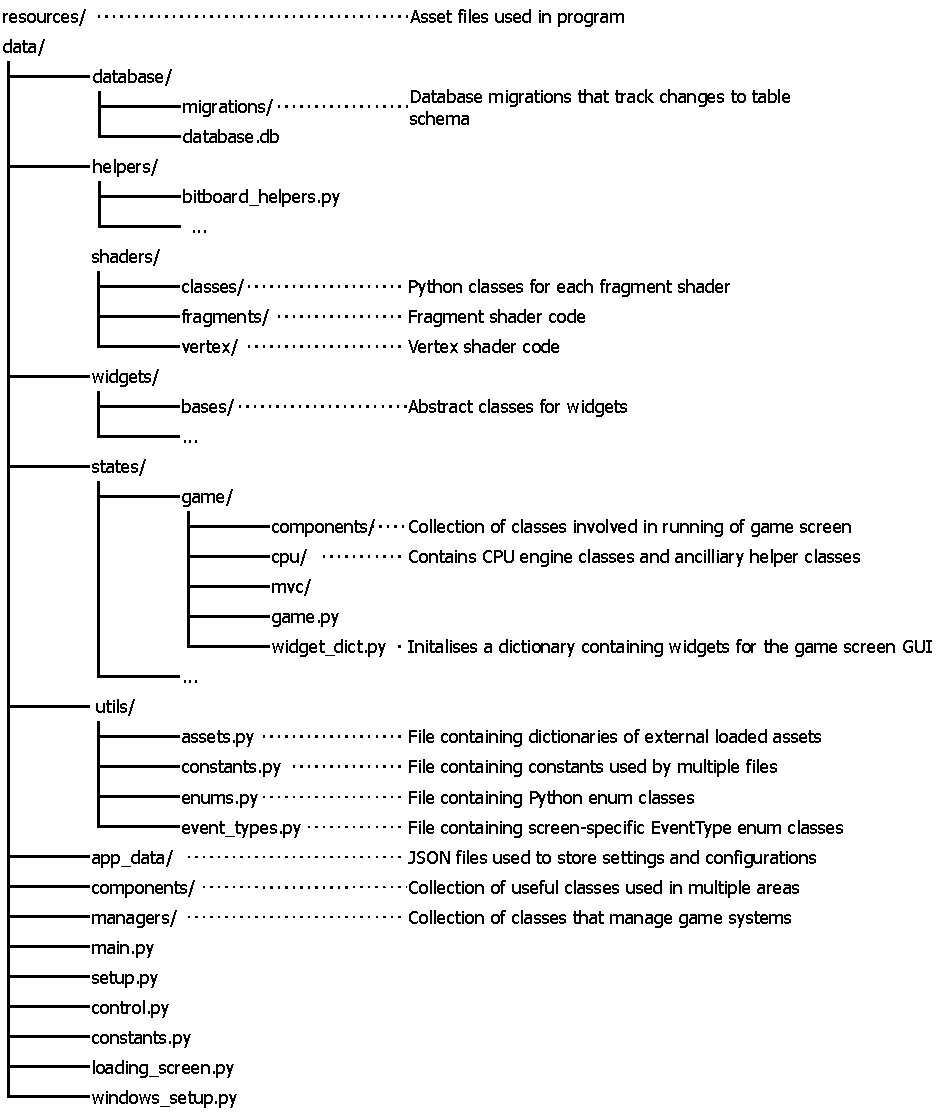
\includegraphics[width=\columnwidth]{../technical_solution/assets/file_tree_diagram.pdf}
    \caption{File tree diagram}
    \label{fig:file-tree-diagram}
\end{figure}

\subsection{Summary of Complexity}
\begin{itemize}
\item Alpha-beta pruning and transposition table improvements for Minimax
\item Shadow mapping and coordinate transformations
\item Recursive Depth-First Search tree traversal
\item Circular doubly-linked list and stack
\item Multipass shaders and gaussian blur
\item Aggregate and Window SQL functions
\item OOP techniques
\item Multithreading (\nameref{sec:loading_screen})
\item Bitboards
\item (Dictionary recursion)
\item (Dot product)
\end{itemize}

\subsection{Overview}

\subsubsection{Main}
The file \lstinline{main.py} is run by the root file \lstinline{run.py}. Here resources-intensive classes such as the state and asset files are initialised, while the program displays a loading screen to hide the loading process. The main game loop is then executed.

\noindent\verb|main.py|
\lstinputlisting{../../data/main.py}

\subsubsection{Loading Screen}
\label{sec:loading_screen}
Multithreading is used to separate the loading screen GUI from the resources intensive actions in \lstinline{main.py}, to keep the GUI responsive. The easing function \lstinline{easeOutBack} is also used to animate the logo.

\noindent\verb|loading_screen.py|
\lstinputlisting{../../data/loading_screen.py}

\subsubsection{Helper functions}
These files provide useful functions for different classes.

\noindent\verb|asset_helpers.py (Functions used for assets and pygame Surfaces)|
\lstinputlisting{../../data/utils/asset_helpers.py}

\bigskip
\noindent\verb|data_helpers.py (Functions used for file handling and JSON parsing)|
\lstinputlisting{../../data/utils/data_helpers.py}


\bigskip
\noindent\verb|widget_helpers.py (Files used for creating widgets)|
\lstinputlisting{../../data/utils/widget_helpers.py}

\subsubsection{Theme}

\subsection{GUI}
\subsubsection{Laser}
\subsubsection{Particles}

\subsection{Game}
\subsubsection{Database}

\end{document}